\documentclass[a4paper,12pt]{article}

\usepackage[utf8]{inputenc}
\usepackage{amsmath}
\usepackage{amssymb}
\usepackage{graphicx}
\usepackage{geometry,pdfpages}
\geometry{a4paper, top=1.5cm,bottom=1.5cm,right=2cm,left=1.5cm}
\usepackage{tikz}
\usetikzlibrary{positioning}
\usetikzlibrary{intersections}
\usetikzlibrary{decorations.markings}
\usetikzlibrary{calc}
\usepackage{pgfplots}
\pgfplotsset{width=9cm, compat=1.9}
\usepackage{multicol}
\usepackage{array}
\usepackage[abs]{overpic}
\usepackage{pict2e}
\renewcommand{\baselinestretch}{1.2}
\setlength{\columnsep}{1cm}
\usepackage[inline]{enumitem}
\usepackage{setspace}
\usepackage{subcaption,tcolorbox}
\usepackage{array}
\usepackage{calc}
\usepackage{tcolorbox}
\usepackage[makeroom]{cancel}
\usepackage{hyperref}
\hypersetup{
	colorlinks=true,
	linkcolor=blue,
	filecolor=magenta,      
	urlcolor=cyan,
} 


\newcolumntype{L}[1]{>{\raggedright\let\newline\\\arraybackslash\hspace{0pt}}m{#1}}
\newcolumntype{C}[1]{>{\centering\let\newline\\\arraybackslash\hspace{0pt}}m{#1}}
\newcolumntype{R}[1]{>{\raggedleft\let\newline\\\arraybackslash\hspace{0pt}}m{#1}}
\usepackage{tcolorbox}
\renewcommand{\arraystretch}{1.5}

\setlength\parindent{0pt}
\newcommand{\lineDist}{1}
\newcommand{\lWid}{0}
\definecolor{linecolor}{RGB}{90,90,90}
\definecolor{shadecolor}{RGB}{180,180,180}
\definecolor{backcolor}{RGB}{220,220,220}
\definecolor{whitening}{RGB}{255,255,255}
\newcommand{\numLines}{2}%subtract one
\newcommand{\Qsep}{1}%separation between Question and lines
%-----------------------------
\newcommand\question{
	\rule[0pt]{17cm}{0.5pt}\vspace{-0.5cm}
	\subsubsection{Exercise}
	
}
\newcommand\questionend{
	\rule[0pt]{17cm}{0.5pt}\vspace{-0.5cm}\\
}
\newcommand\quiz{
	\subsubsection{Quiz}\vspace{-0.5cm}
}

\newcommand\boxes[7]{
	\begin{tikzpicture}
		\newcommand{\wid}{1.6cm}
		\newcommand{\hgt}{1cm}
		\newcommand{\brd}{0.4cm}
		\draw[](0,0)rectangle(0+\wid,0+\hgt);
		\draw[](\wid/2,\hgt/2)node[]{\footnotesize #1};
		\draw[](0-\wid/2,0-\hgt)rectangle(0+\wid/2,0);
		\draw[](0,-\hgt/2)node[]{\footnotesize #2};
		\draw[](0+\wid/2,0-\hgt)rectangle(0+3*\wid/2,0);
		\draw[](\wid,-\hgt/2)node[]{\footnotesize #3};
		\draw[](0-\wid,0-2*\hgt)rectangle(0,-\hgt);
		\draw[](-\wid/2,-3*\hgt/2)node[]{\footnotesize #4};
		\draw[](0,0-2*\hgt)rectangle(\wid,-\hgt);
		\draw[](\wid/2,-3*\hgt/2)node[]{\footnotesize #5};
		\draw[](0+\wid,0-2*\hgt)rectangle(2*\wid,-\hgt);
		\draw[](3*\wid/2,-3*\hgt/2)node[]{\footnotesize #6};
		\draw[white](-\wid-\brd,-2*\hgt-\brd)rectangle(2*\wid+\brd,\hgt+\brd);
		\draw[](-\wid-\brd,\hgt+\brd)node[anchor= north west]{\textbf{#7)}};
	\end{tikzpicture}
}

\newcommand\boxesSol[7]{
	\begin{tikzpicture}
		\newcommand{\wid}{1.6cm}
		\newcommand{\hgt}{1cm}
		\newcommand{\brd}{0.4cm}
		\draw[](0,0)rectangle(0+\wid,0+\hgt);
		\draw[](\wid/2,\hgt/2)node[]{\footnotesize #1};
		\draw[](0-\wid/2,0-\hgt)rectangle(0+\wid/2,0);
		\draw[](0,-\hgt/2)node[]{\footnotesize #2};
		\draw[](0+\wid/2,0-\hgt)rectangle(0+3*\wid/2,0);
		\draw[](\wid,-\hgt/2)node[]{\footnotesize #3};
		\draw[](0-\wid,0-2*\hgt)rectangle(0,-\hgt);
		\draw[](-\wid/2,-3*\hgt/2)node[]{\footnotesize #4};
		\draw[](0,0-2*\hgt)rectangle(\wid,-\hgt);
		\draw[](\wid/2,-3*\hgt/2)node[]{\footnotesize #5};
		\draw[](0+\wid,0-2*\hgt)rectangle(2*\wid,-\hgt);
		\draw[](3*\wid/2,-3*\hgt/2)node[]{\footnotesize #6};
		\draw[white](-\wid-\brd,-2*\hgt-\brd)rectangle(2*\wid+\brd,\hgt+\brd);
		\draw[](-\wid-\brd,\hgt+\brd)node[anchor= north west]{\textbf{#7)}};
	\end{tikzpicture}
}

\newcommand\addagon[7]{
	\begin{tikzpicture}[scale=1]
		\draw[white](-3,0)rectangle(3,5.5);
		\draw[](-3,4)node[right]{#7)};
		\begin{scope}[scale=0.75]
			\coordinate (A) at (-2.5,1);
			\coordinate (B) at (2.5,1);
			\coordinate (C) at (0,{2.5*sqrt(3)+1});
			\draw[thick](A)--(B)--(C)--(A);
			\foreach \n in {A,B,C}{
				\filldraw[fill=white, draw=black](\n )circle[radius=1cm];
			}
			\draw[](A)node[above, yshift=-9pt]{#1};
			\draw[](B)node[above, yshift=-9pt]{#2};
			\draw[](C)node[above, yshift=-9pt]{#3};
			
			\coordinate (A') at ( $ (A)!0.5!(B) $ );
			\draw[fill=backcolor, draw=black]([shift=(35:-1.2)]A')rectangle([shift=(35:1.2)]A');
			\draw[](A')node[above, yshift=-9pt]{#4};
			
			\coordinate (B') at ( $ (B)!0.5!(C) $ );
			\draw[fill=backcolor, draw=black]([shift=(35:-1.2)]B')rectangle([shift=(35:1.2)]B');
			\draw[](B')node[above, yshift=-9pt]{#5};
			
			\coordinate (C') at ( $ (C)!0.5!(A) $ );
			\draw[fill=backcolor, draw=black]([shift=(35:-1.2)]C')rectangle([shift=(35:1.2)]C');
			\draw[](C')node[above, yshift=-9pt]{#6};
		\end{scope}
	\end{tikzpicture}
}

\newcommand\addagonSol[7]{
	\begin{tikzpicture}[scale=1]
		\draw[white](-3,0)rectangle(3,5.5);
		\draw[](-3,4)node[right]{#7)};
		\begin{scope}[scale=0.75]
			\coordinate (A) at (-2.5,1);
			\coordinate (B) at (2.5,1);
			\coordinate (C) at (0,{2.5*sqrt(3)+1});
			\draw[thick](A)--(B)--(C)--(A);
			\foreach \n in {A,B,C}{
				\filldraw[fill=white, draw=black](\n )circle[radius=1cm];
			}
			\draw[](A)node[above, yshift=-9pt]{#1};
			\draw[](B)node[above, yshift=-9pt]{#2};
			\draw[](C)node[above, yshift=-9pt]{#3};
			
			\coordinate (A') at ( $ (A)!0.5!(B) $ );
			\draw[fill=backcolor, draw=black]([shift=(35:-1.2)]A')rectangle([shift=(35:1.2)]A');
			\draw[](A')node[above, yshift=-9pt]{#4};
			
			\coordinate (B') at ( $ (B)!0.5!(C) $ );
			\draw[fill=backcolor, draw=black]([shift=(35:-1.2)]B')rectangle([shift=(35:1.2)]B');
			\draw[](B')node[above, yshift=-9pt]{#5};
			
			\coordinate (C') at ( $ (C)!0.5!(A) $ );
			\draw[fill=backcolor, draw=black]([shift=(35:-1.2)]C')rectangle([shift=(35:1.2)]C');
			\draw[](C')node[above, yshift=-9pt]{#6};
		\end{scope}
	\end{tikzpicture}
}


\newcommand\sumproduct[5]{
	\begin{tikzpicture}[scale=0.6]
		\draw[white](-4.75,-2.75)rectangle(4.75,5);
		\draw[](-4.5,4.5)node[right, yshift=-0.2cm]{\footnotesize \textbf{#5)}};
		\draw[](-4,0)rectangle(0,2);
		\draw[](0,0)rectangle(4,2);
		\draw[](-2,2)rectangle(2,4);
		\draw[](-2,-2)rectangle(2,0);
		\draw[](0,-1)node[]{#1};
		\draw[](0,3)node[]{#2};
		\draw[](-2,1)node[]{#3};
		\draw[](2,1)node[]{#4};
		\draw[](-4,3)node[right]{\tiny Product:};
		\draw[](-4,-1)node[right]{\tiny Sum:};
	\end{tikzpicture}
}
\newcommand\sumproductSol[5]{
	\begin{tikzpicture}[scale=0.6]
		\draw[white](-4.75,-2.75)rectangle(4.75,5);
		\draw[](-4.5,4.5)node[right, yshift=-0.2cm]{\footnotesize \textbf{#5)}};
		\draw[](-4,0)rectangle(0,2);
		\draw[](0,0)rectangle(4,2);
		\draw[](-2,2)rectangle(2,4);
		\draw[](-2,-2)rectangle(2,0);
		\draw[](0,-1)node[]{#1};
		\draw[](0,3)node[]{#2};
		\draw[](-2,1)node[]{#3};
		\draw[](2,1)node[]{#4};
		\draw[](-4,3)node[right]{\tiny Product:};
		\draw[](-4,-1)node[right]{\tiny Sum:};
	\end{tikzpicture}
}


\begin{document}
	\section*{Extension activities}
	\subsection*{Power of zero and negative powers}
	Evaluate the powers given to gain an intuitive understanding of what a power of zero means and what a negative power means.\\\\
	\renewcommand{\arraystretch}{1.5}
		\begin{tabular}{*{8}{|C{1.75cm}}|}\hline
		$2^4$&$2^3$&$2^2$&$2^1$&$2^0$&$2^{-1}$&$2^{-2}$&$2^{-3}$\\\hline
		& & & & & & &  \\
		& & & & & & &  \\\hline
	\end{tabular}\vspace{1cm}\\
	
	\begin{tabular}{*{8}{|C{1.75cm}}|}\hline
$3^4$&$3^3$&$3^2$&$3^1$&$3^0$&$3^{-1}$&$3^{-2}$&$3^{-3}$\\\hline
& & & & & & &  \\
	& & & & & & &  \\\hline
\end{tabular}\vspace{0.5cm}\\

From this we can deduce some rules for exponents:
\begin{align*}
x^0 &= 1\\
x^{-n}& = \frac{1}{x^n}
\end{align*}
we also have:
\begin{align*}
	x^m\times x^n &= x^{m+n}\\
	(x^m)^n &= x^{mn}
\end{align*}
and can show:
\begin{align*}
	\frac{x^m}{x^n}&=\frac{x^m}{1} \times \frac{1}{x^n} \\
	&=x^m \times x^{-n} = x^{m-n}
\end{align*}
\questionend
\newpage
\subsubsection*{Questions}
\begin{enumerate}[label=\normalsize \arabic*)~~~ , leftmargin=1cm]
	\item Simplify
\begin{multicols}{2}
	\begin{enumerate}[label=\normalsize \alph*)~~~ ,  topsep=8pt,itemsep=5pt,partopsep=4pt, parsep=4pt]
		\item $(2x)^0$
		\item $3x^0$
		\item $(-5)^0$
		\item $x \times 4x^0$
	\end{enumerate}
\end{multicols}
\questionend
\item Simplify and write with positive exponents:
\begin{multicols}{3}
	\begin{enumerate}[label=\normalsize \alph*)~~~ , topsep=8pt,itemsep=5pt,partopsep=4pt, parsep=4pt]
		\item $x^{-2}$
		\item $3x^{-2}$
		\item $x^3 \times x^{-2}$
		\item $x^4 \times x^{-5}$
		\item $y \times y^{-5}$
		\item $3x^{-1} \times y$
			\item $4y^{-2} \times 3y^{-1}$
		\item $7x^{-1} \times y^{-3}$
		\item $3x^{2}y \times 2xy^{-3}$
	\end{enumerate}
\end{multicols}
\questionend
\item Simplify and write with positive exponents:
\begin{multicols}{3}
	\begin{enumerate}[label=\normalsize \alph*)~~~ , topsep=8pt,itemsep=5pt,partopsep=4pt, parsep=4pt]
		\item $(3x)^{-2}$
		\item $(3x)^{-2} \times x^4$
		\item $(7x)^2 \times x^{-2}$
		\item $(3x)^{-2} \times x^{-2}$
		\item $(4xy)^2 \times (xy)^{-3}$
		\item $9x^{-2} \times (3x)^{-1}$
		\item $4^2x^{-3} \times 4^{-1}xy$
		\item $3x^{-1} \times (y^{-2})^{-1}$
		\item $(y^{-2})^{-3} \times x^{-3}$
	\end{enumerate}
\end{multicols}
\questionend
\item Evaluate these fractions:
\begin{multicols}{4}
	\begin{enumerate}[label=\normalsize \alph*)~~~ , topsep=8pt,itemsep=5pt,partopsep=4pt, parsep=4pt]
			\item $\displaystyle \frac{~~1~~}{ \frac{1}{2} }$
				\item $\displaystyle \frac{~~3~~}{ \frac{1}{2} }$
		\item $\displaystyle \frac{~~1~~}{ \frac{2}{3} }$
		\item $\displaystyle \frac{~~\frac{3}{2}~~}{ \frac{2}{3} }$
		\item $\displaystyle \frac{~~~1~~~}{ 2^{-1}}$
		\item $\displaystyle \frac{~~~1~~~}{ 2^{-2}}$
		\item $\displaystyle \left( \frac{1}{ 3} \right)^{-1} $
		\item $\displaystyle \left( \frac{2}{ 3} \right)^{-2} $
	\end{enumerate}
\end{multicols}
\questionend
\item Simplify and write with positive exponents:
\begin{multicols}{3}
	\begin{enumerate}[label=\normalsize \alph*)~~~ , topsep=8pt,itemsep=5pt,partopsep=4pt, parsep=4pt]
	\item $\displaystyle \frac{1}{x^{-2}}$
\item$\displaystyle \left( \frac{1}{x} \right)^{-2}$
\item$\displaystyle \left( \frac{y}{x} \right)^{-2}$
\item$\displaystyle \left( \frac{yx^3}{x^2} \right)^{-2}$
\item$\displaystyle \left( \frac{3x^4}{y} \right)^{-3}$
\item$\displaystyle \left( \frac{6x^2}{3x^2y} \right)^{-1}$
	\end{enumerate}
\end{multicols}
\end{enumerate}
\newpage
\subsection*{Fractional powers}
The square root of the number $x$ is the (positive) number $y$ such that $y^2 = x$.\\
For example: $\sqrt{25} = 5$ because $5^2 = 25$.\\
Please note that $-5 \times -5 = 25$ but the square root function $\sqrt{25}$ only returns a positive value.
\questionend
\begin{enumerate}[label=\normalsize \arabic*)~~~ , leftmargin=1cm]
\item Evaluate the following
\begin{multicols}{3}
	\begin{enumerate}[label=\normalsize \alph*)~~~ , topsep=8pt,itemsep=5pt,partopsep=4pt, parsep=4pt]
		\item $\displaystyle \sqrt{4} $
		\item $\displaystyle  \sqrt{64}  $
		\item $\displaystyle \sqrt{49}  $
		\item $\displaystyle \sqrt{ \frac{25}{ 9 } }$
		\item $\displaystyle \sqrt{ \frac{121}{ 169 } }$
		\item $\displaystyle \sqrt{a^2}$
		\item $\displaystyle \sqrt{a^4}$
		\item $\displaystyle \sqrt{a^6}$
		\item $\displaystyle \sqrt{a^2b^6 }$
			\item $\displaystyle \sqrt{ \frac{9x^4}{y^8} }$
				\item $\displaystyle \sqrt{ \frac{16x^3y^2}{xy^4} }$
	\end{enumerate}
\end{multicols}
\item Evaluate the following
\begin{multicols}{3}
	\begin{enumerate}[label=\normalsize \alph*)~~~ , topsep=8pt,itemsep=5pt,partopsep=4pt, parsep=4pt]
		\item $\displaystyle \sqrt{4} \times \sqrt{4} $
		\item $\displaystyle  \sqrt{a} \times \sqrt{a}   $
		\item $\displaystyle (\sqrt{a^2})^3  $
		\item $\displaystyle (3b\sqrt{a})^2  $
		\item $\displaystyle\sqrt{xy} \times \sqrt{xy}$
		\item $\displaystyle (4\sqrt{a^2})^3$
	\end{enumerate}
\end{multicols}
\end{enumerate}
\questionend

We can now see that:
\begin{align*}
	\sqrt{x} \times \sqrt{x} = x\\
	x^{\frac{1}{2}} \times x^{\frac{1}{2}}  = x^1 = x
\end{align*}
Which tells us that:
\begin{align*}
x^{\frac{1}{2}}  = \sqrt{x}
\end{align*}
And it is probably good to note that the addition, subtraction and power rules still hold:
\begin{align*}
	x^{\frac{1}{2}} \times x^{2}   = x^{\frac{1}{2} + 2} = x^{ \frac{5}{2}  }\\
		\frac{ x^{ \frac{7}{2} }  }{ x^{  \frac{1}{2} }  }  = x^{ \frac{7}{2} -  \frac{1}{2} } = x^{3}\\
		(9b)^{ \frac{1}{2} }= 9^{ \frac{1}{2} } \times b^{ \frac{1}{2} } = 3\sqrt{b}
\end{align*}

\questionend
\newpage

\begin{enumerate}[label=\normalsize \arabic*)~~~ , leftmargin=1cm]
	\setcounter{enumi}{2}
\item Simplify:
\begin{multicols}{3}
	\begin{enumerate}[label=\normalsize \alph*)~~~ , topsep=8pt,itemsep=5pt,partopsep=4pt, parsep=4pt]
		\item $\displaystyle \left(16b^4 \right)^{ \frac{1}{2} } $
		\item  $\displaystyle \left(81^{\frac{1}{2}} b^4 \right)^{ \frac{1}{2} } $
		\item  $\displaystyle \sqrt{100a^2b^{10}} $
		\item $\displaystyle \left(  \frac{1}{16x^4} \right)^\frac{1}{2}  $
		\item $\displaystyle  \left(  \frac{108x^2y^6}{3x^4} \right)^\frac{1}{2} $
		\item $\displaystyle  \sqrt{ \frac{256y^6}{x^{12}} }$
	\end{enumerate}
\end{multicols}
\end{enumerate}

\questionend

Looking at the power rule we can note:
\begin{align*}
	9^{\frac{3}{2}} = \left( 9^{ \frac{1}{2} } \right)^3 = 3^3 = 27
\end{align*}

\questionend

\begin{enumerate}[label=\normalsize \arabic*)~~~ , leftmargin=1cm]
		\setcounter{enumi}{3}
\item Evaluate without a calculator (use a calculator afterwards to check your work and make sure you can enter the powers correctly)
\begin{multicols}{4}
	\begin{enumerate}[label=\normalsize \alph*)~~~ , topsep=8pt,itemsep=5pt,partopsep=4pt, parsep=4pt]
		\item $\displaystyle 4^{ \frac{5}{2} } $
		\item  $\displaystyle 16^{ \frac{3}{2} } $
		\item  $\displaystyle100^{ \frac{7}{2} }$
		\item $\displaystyle 36^{ \frac{3}{2} } $
	\end{enumerate}
\end{multicols}
\questionend
\item Simplify, by writing with no brackets, some powers will stay as fractions
\begin{multicols}{2}
	\begin{enumerate}[label=\normalsize \alph*)~~~ , topsep=8pt,itemsep=5pt,partopsep=4pt, parsep=4pt]
			\item $\displaystyle \left( 3^4xy^2 \right)^{ \frac{1}{2} } \times 4y^2 $
			\item  $\displaystyle \frac{5^2a}{b^4} \times \frac{b ^ {\frac{3}{2}}}{a} $
			\item  $\displaystyle \left( \frac{x}{ x^\frac{1}{2} } \right)^3$
			\item $\displaystyle \left( xy \right)^\frac{1}{2} \times x^{ -\frac{5}{2} }  $
			\item $\displaystyle  \left(  5^\frac{3}{2}  x^{ \frac{5}{2}  } y^3 \right)^2$
			\item $\displaystyle  \left( \sqrt{ \frac{x}{2} }~ \right)^3$
			\item $\displaystyle  \sqrt{   \left(   \frac{x}{2}  \right) ^3   }$
	\end{enumerate}
\end{multicols}
\questionend
\item Bit of review, simplify:
\begin{multicols}{3}
	\begin{enumerate}[label=\normalsize \alph*)~~~ , topsep=8pt,itemsep=5pt,partopsep=4pt, parsep=4pt]
		\item $\displaystyle\sqrt{16x^{16}}$\\
		\item $\displaystyle\sqrt{36x^{36}}$\\
		\item $\displaystyle\frac{4m^8}{\sqrt{36m^{20}}}$\\
		\item $\displaystyle\frac{\sqrt{9n^{4}}}{3n^2}$\\
		\item $\displaystyle\frac{(3a^2b^2)^4}{27 a^8b^9}$\\ 
		\item $\displaystyle (0.25 x^3)^\frac{1}{2}$\\
		\item $\displaystyle \frac{(4a^2)^3}{(8a^5)^2}$\\  
		\item $\displaystyle \sqrt{\frac{256 a^{16}}{b^{12}}}$\\
	\end{enumerate}
\end{multicols}\vspace{1cm}

\end{enumerate}
\newpage
\subsection*{Algebraic fractions}
\begin{figure}[!h]
	\centering
	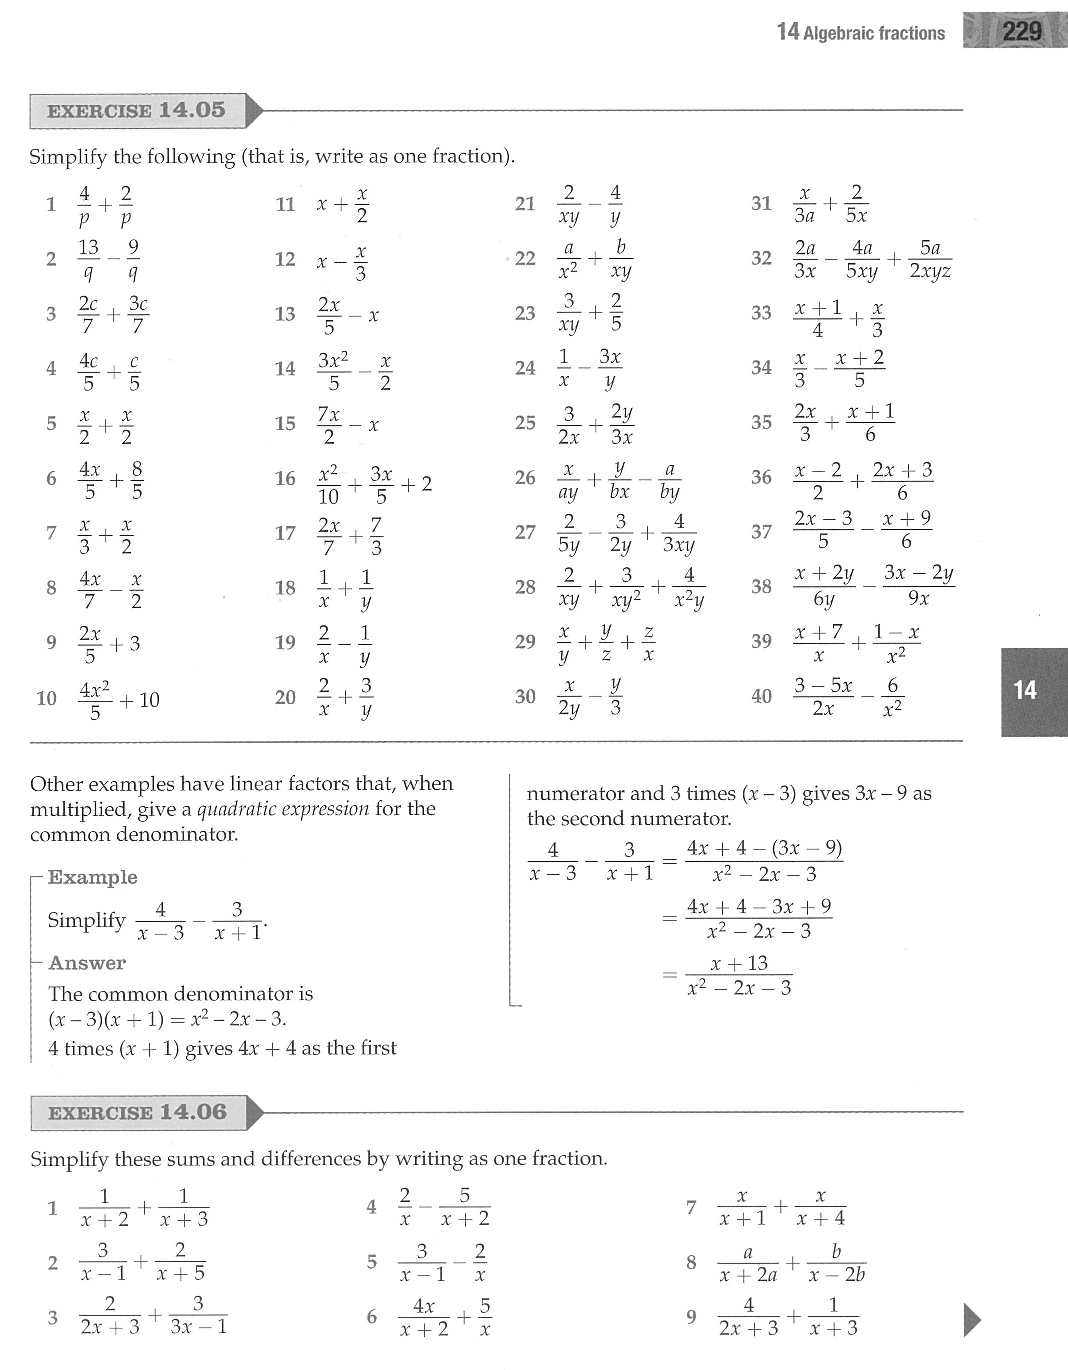
\includegraphics[width=18cm]{Theta_set1}
\end{figure}
\newpage
\begin{figure}[!h]
	\centering
	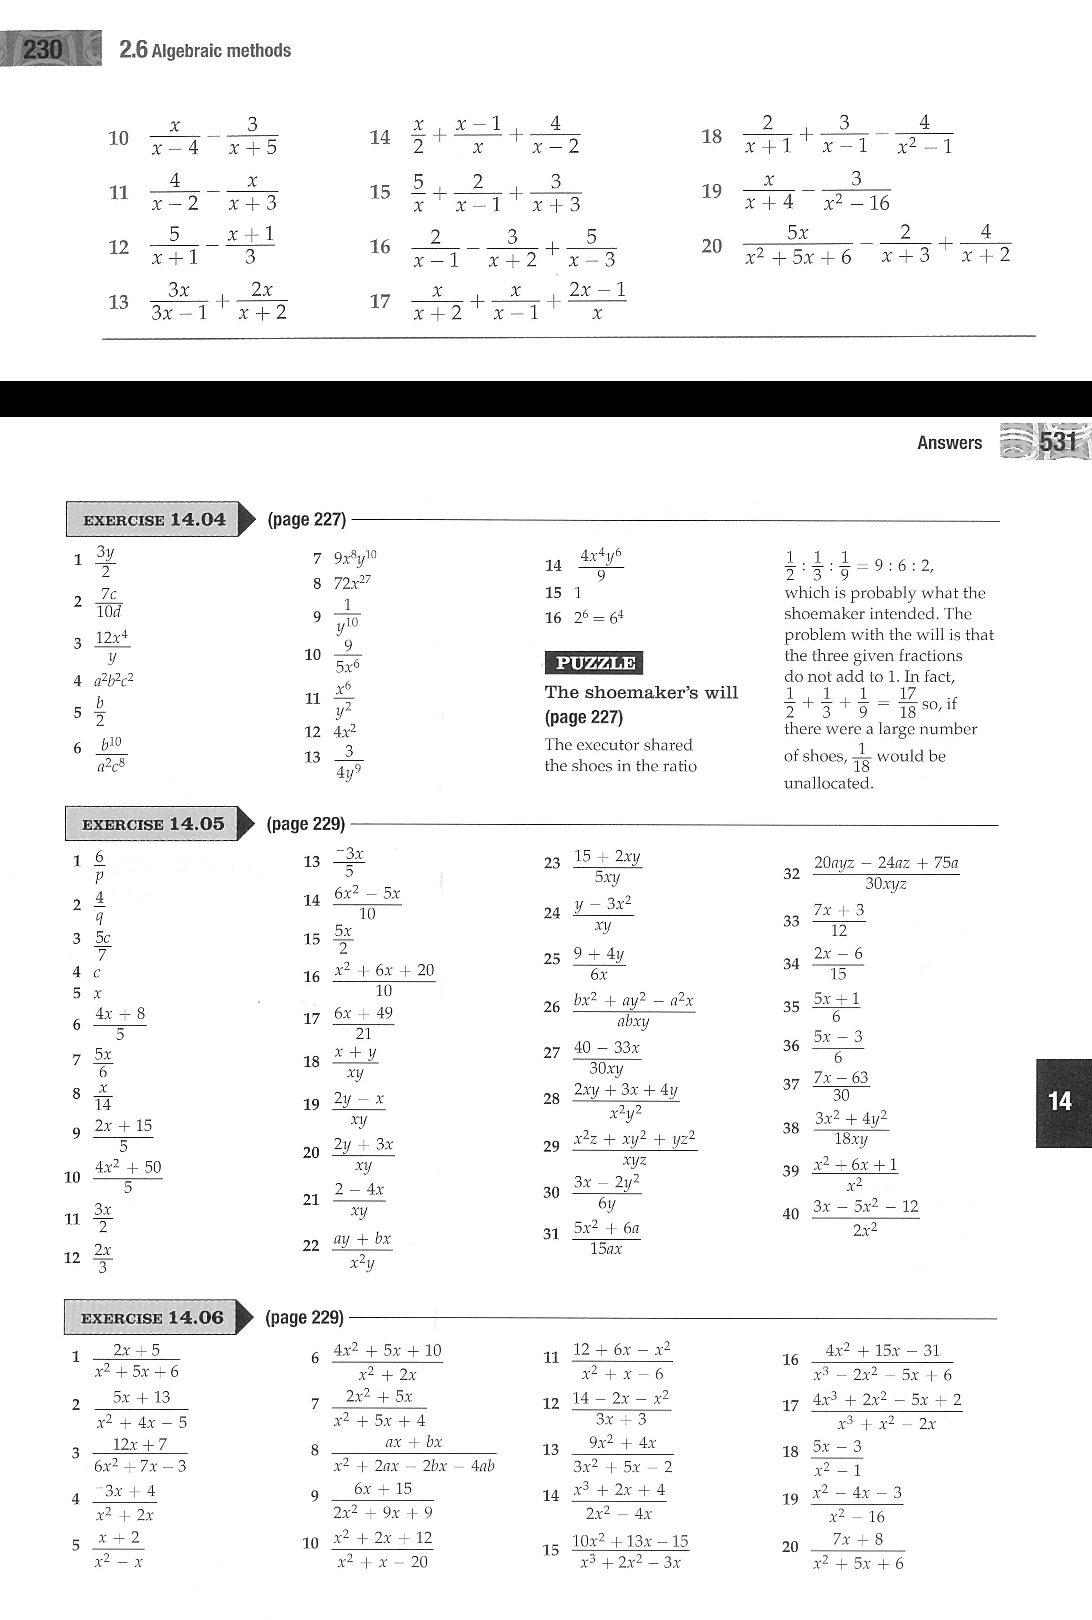
\includegraphics[width=18cm]{Theta_set2}
\end{figure}



\end{document}